\documentclass[11pt]{article}
\title{\textbf{Using the Invoice Class}}
\author{\textbf{Alan Munn}\\Department of Linguistics and Languages\\\texttt{\href{mailto:amunn@msu.edu}{amunn@msu.edu}}}
\date{Version 1.0\\January 17, 2019}
\usepackage{fontspec}
\setmainfont[]{Linux Libertine O}
\setsansfont[]{Linux Biolinum O}
\setmonofont[Scale=MatchLowercase]{Linux Libertine Mono O}
\usepackage[lmargin=1in,rmargin=1in,tmargin=1.25in,bmargin=1in]{geometry}
\usepackage{titling}
\usepackage{array, booktabs, multicol, xspace,tabularx}
\usepackage{enumitem}
\usepackage{caption}
\usepackage{fancyvrb,listings,url}
\usepackage{pdfpages}
\usepackage[sf]{titlesec}
\usepackage{titleps}
\newpagestyle{main}{%
\setfoot{\itshape Invoice Class}{}{\thepage}}
\pagestyle{main}

\usepackage[colorlinks=true]{hyperref}

\DefineShortVerb{\|}
\newcommand*\bs{\textbackslash}
  
\lstset{%
    basicstyle=\ttfamily\small,
    commentstyle=\itshape\ttfamily\small,
    showspaces=false,
    showstringspaces=false,
    breaklines=true,
    breakautoindent=true,
    frame=single
    captionpos=t
    language=TeX
}
  
\newcommand*{\pkg}[1]{\texttt{#1}\xspace}
\setitemize[1]{label={}}
\setitemize[2]{label={}}
\setdescription{font={\normalfont}}
\setlength{\droptitle}{-1in}



\begin{document}
\maketitle
\thispagestyle{empty}
\section{Introduction}
The \pkg{invoice-class} class allows printing of a standard US commercial invoice using invoice data from a CSV spreadsheet. Invoices can span multiple pages.

\section{Class document commands}
The main class commands specify the parts of the form that need to be filled in.  Each command except |\weight| takes a single argument.

\begin{center}
\begin{tabularx}{.8\textwidth}{>{\ttfamily\bs}l<{\{\}}X}
\toprule
\multicolumn{1}{c}{Command name} & \multicolumn{1}{l}{Description}\\
\midrule
{waybill}& waybill number\\
{shippingdate}& shipping date (default is \texttt{\bs today})\\
{carrier}& name of the freight carrier\\
{destination}& destination country\\
{toaddress}& Destination address\\
\multicolumn{1}{>{\ttfamily\bs}l}{weight\{<lbs>\}\{<oz>\}} & weight in pounds and ounces\\
{packages}{1} & number of packages in the shipment\\
{shippingcost}& total cost of shipping (default = 0.00)\\
{packingcost} & total cost of packing (default = 0.00)\\
{insurancecost} & total cost of insurance (default is 0.00)\\
{InputFile} & name of the CSV file for item date\\
\bottomrule
\end{tabularx}
\captionof{table}{Invoice document commands}\label{commands}
\end{center}

\subsection{Producing the invoice}
Once all the required elements  are specified (which can be done in the preamble), there is a single command to produce the invoice:
\begin{center}
\begin{tabularx}{.8\textwidth}{>{\ttfamily\bs}lX}
{printinvoice} & Prints the invoice\\
\end{tabularx}
\end{center}

\section{Class configuration commands}
Since an invoice will generally have a fixed From address, shipper and location, these values are best set in a separate configuration file (although they can also be set within the document.) The class will look for the file |invoice.cfg| or, |<prefix>invoice.cfg| where |<prefix>| is specified using the document command |\ConfigPrefix|. This allows multiple configuration files with different information within them.
Each configuration file should contain an instance of |\fromaddress|, |\shipper|, and |\location|.
\begin{center}
\begin{tabularx}{.8\textwidth}{>{\ttfamily\bs}l<{\{\}}X}
\toprule
\multicolumn{1}{c}{Command name} & \multicolumn{1}{l}{Description}\\
\midrule
{fromaddresss}& shipper's address\\
{shipper}& name of shipper\\
{location}& location\\
{ConfigPrefix} & configuration file prefix (default is none)\\
\bottomrule
\end{tabularx}
\captionof{table}{Invoice configuration commands}\label{config-commands}
\end{center}


\section{\pkg{datatool} details}
The uses the \pkg{datatool} package to produce the invoice using a CSV file. The CSV file requires the following column headings to be present. All other columns are ignored. (Heading names are case-sensitive.)
\begin{center}
\begin{tabularx}{.8\textwidth}{>{\ttfamily}lX}
\toprule
\multicolumn{1}{c}{Column name} & \multicolumn{1}{l}{Description}\\
\midrule
{Description} &  Item description\\
{Country} & Country of origin\\
{Quantity} & unit quantity\\
{UnitValue} & per unit value\\
{Amount} & total value for item\\
\bottomrule
\end{tabularx}
\captionof{table}{Required CSV Column labels}\label{CSV}
\end{center}
\subsection{Sample CSV file}
\lstinputlisting{ducks.csv}
\clearpage
\section{Sample Configuration file}
\lstinputlisting{duck-invoice.cfg}

\section{Sample document}
\lstinputlisting{ducks.tex}
\section{Bugs and support}
This package is released as is, and although I will accept bug reports, fixing them may not be a priority. You're free to fork the project to modify it as you wish.


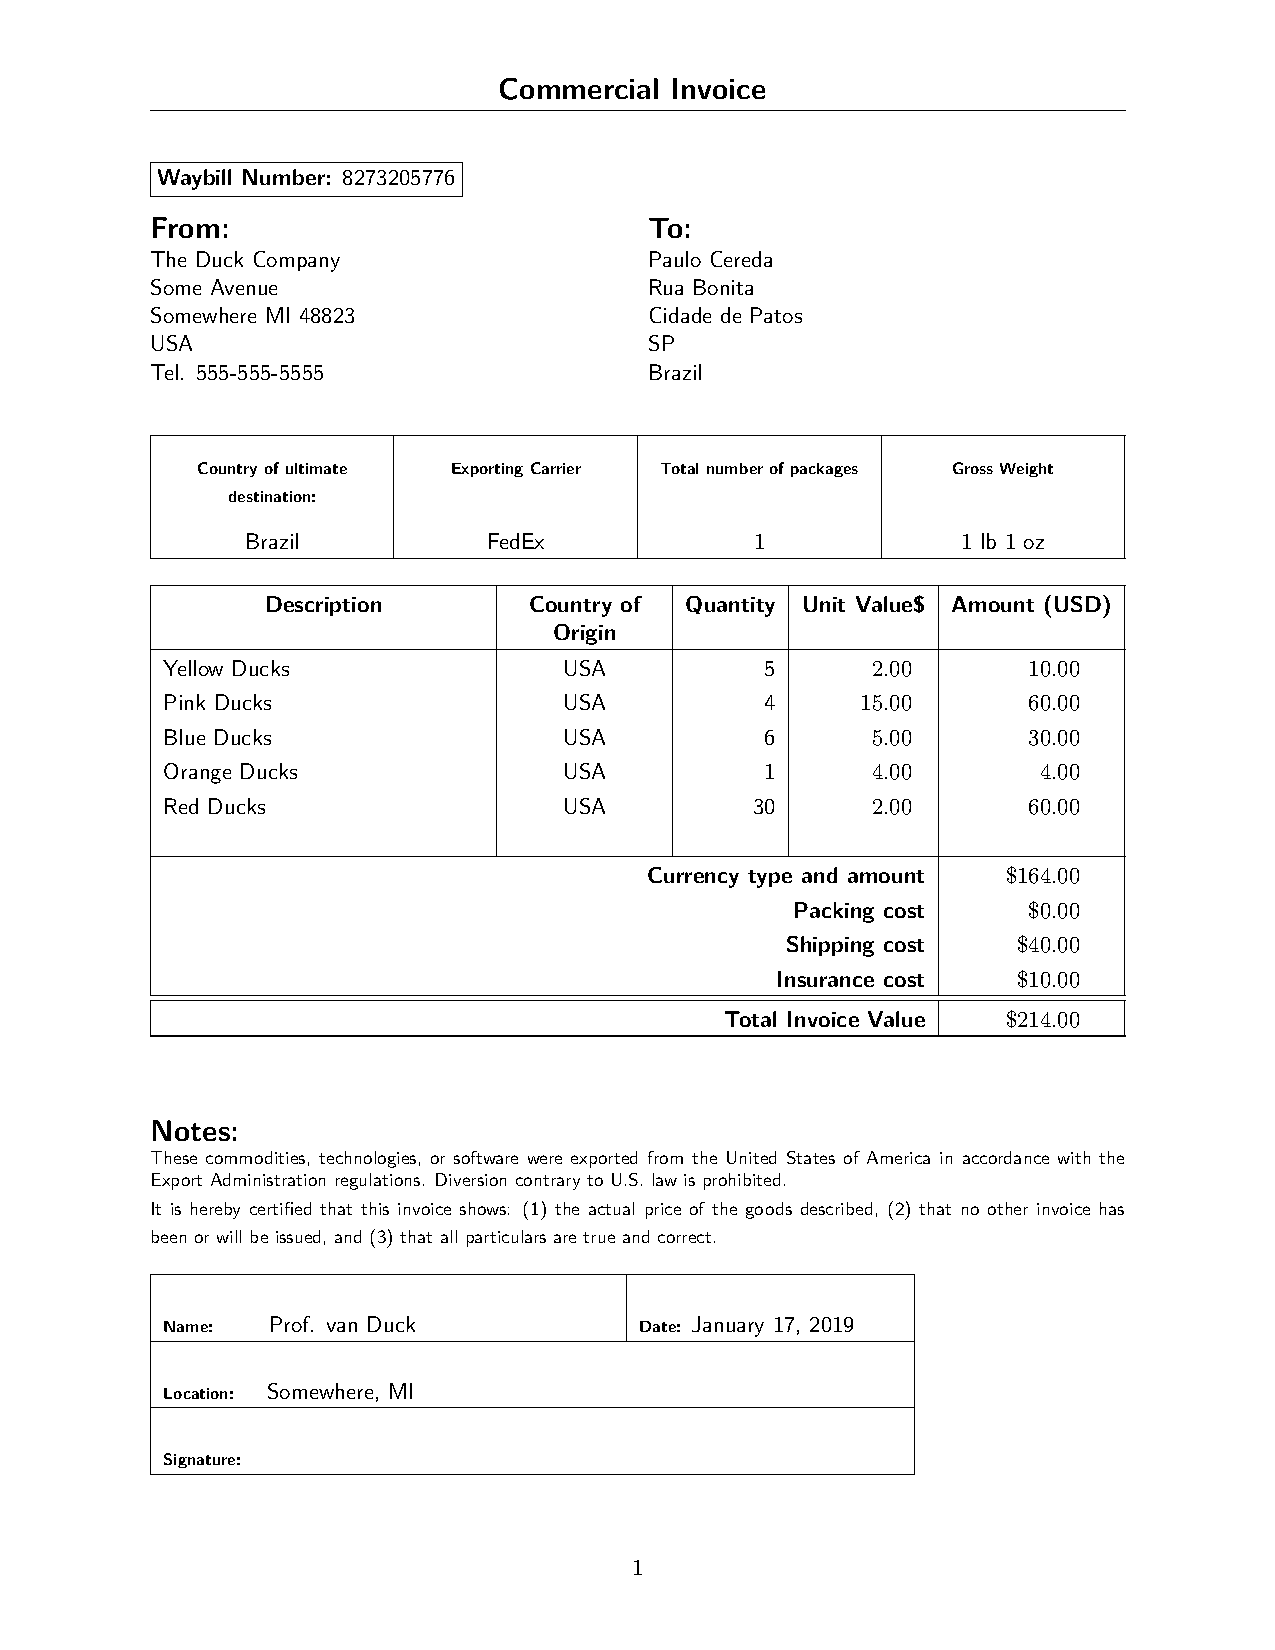
\includepdf[]{ducks.pdf}
\end{document}
